\documentclass[a4paper]{article}
\usepackage[utf8]{inputenc}
\usepackage[T1]{fontenc}
\usepackage{lmodern}
\usepackage{listings}
\usepackage{graphicx}
\usepackage{dirtree}
\usepackage{caption}
\usepackage{subcaption}
\usepackage{float}
\usepackage[english]{babel}
\usepackage[margin=1.1in]{geometry}
\title{Human Intracranial Brain Observations Player \\ User Manual}
\author{\textsc{BONTEMPS Benjamin} \\ \textsc{CHATARD Benoît} \\ \textsc{GANNERIE Adrien}}
\lstset{
	frame = single,
	basicstyle = \footnotesize\ttfamily
}

\begin{document}
\maketitle
\begin{abstract}
This document is the user manual of the Human Intracranial Brain Observations Player (HiBoP). HiBoP is being developed by the Centre de Recherche en Neurosciences de Lyon (CRNL), with funds from the Human Brain Project (HBP) to visualize large datasets of intracranial electroencephalography (iEEG) data. This document was written for the 2.1.0 version of HiBoP.
\end{abstract}
\tableofcontents
\section{HiBoP project} \label{data}
\paragraph{} A \textbf{Project} links together anatomical and functional data from a set of patients. If you have an anatomical description of the patients (3D mesh of the brain, MRI and coordinates of the sites of the electrodes) and the respective iEEG data, you can visualize them in 4D (3D space + time). The first thing to do with HiBoP is to create or open a Project. This can be done within HiBoP (section \ref{UI}), but also using a third-party software which automatically generates the files and the hierarchy, such as the HiBoP Database Manager (appendix \ref{bddmanager}).
\paragraph{} On your Hard Drive, the Project consists of a .hibop file. This file is in reality a zip archive containing several subfolders (Figure \ref{projectDirectory}). The contents of this archive can be extracted using an unzipping software. Each file is encoded with the json format, and thus can be edited (at your own risks) using any text editor. However this is not recommended, as any coma missing may cause the file to be incorrectly interpreted. You can then zip the folder again and rename the extension from .zip to .hibop.
\begin{figure}[H]
\framebox[\textwidth]{%
\begin{minipage}{0.9\textwidth}
\dirtree{%
	.1 ProjectName.hibop/.
	.2 ProjectName.settings.
	.2 Datasets/.
	.3 DatasetName.dataset.
	.3 ....
	.2 Groups/.
	.3 GroupName.group.
	.3 ....
	.2 Patients/.
	.3 PatientName.patient.
	.3 ....
	.2 Protocols/.
	.3 ProtocolName.prov.
	.3 ....
	.3 Icons/.
	.4 Icon1.png.
	.4 Icon2.jpg.
	.4 ....
	.2 Visualizations/.
	.3 VisualizationName.visualization.
	.3 ....
}
\end{minipage}
}
\caption{\label{projectDirectory}Project directory hierarchy}
\end{figure}
\subsection{Settings}
\paragraph{} The .settings file at the root of the project archive describes some project settings (Figure \ref{projectSettings}). This file contains the name of the project, a default path for the anatomical data of the patients and a default path for the functional data (iEEG), as well as aliases to shorten paths in other files.
\begin{figure}[H]
\begin{lstlisting}
{
  "ID": "41001a8a-23a5-409b-8b87-099dbb727a18",
  "Name": "ProjectName",
  "PatientDatabase": "Y:/BrainVisaDB/Epilepsy",
  "LocalizerDatabase": "Y:/LOCA_DATABASE",
  "Aliases": [
    {
      "Key": "[PATIENT_DATABASE]",
      "Value": "Y:/BrainVisaDB/Epilepsy"
    },
    {
      "Key": "[LOCALIZERS_DATABASE]",
      "Value": "Y:/LOCA_DATABASE"
    }
  ]
}
\end{lstlisting}
\caption{\label{projectSettings}Example project settings file}
\end{figure}
\subsection{Patients}
\paragraph{} This subfolder contains .patient files, which contains metadata of the patients and full paths towards anatomical files for each patient (Figure \ref{patientFile}). A 3D mesh can be a single mesh (only one file) or a left-right mesh (one file for the left part and one for the right part of the brain). These files are in GIfTI format (.gii). You can also provide aditional files to show MarsAtlas parcels (.gii), or a transformation file (to align the mesh and its respective MRI, .trm). The MRIs must be in the NIfTI-1 format (.nii). The implantations must be in the PTS format. The connectivities files are CCEP (amplitude / latencies) text files.
\begin{figure}[H]
\begin{lstlisting}
{
  "ID": "LYONNEURO_2013_CHAj",
  "Name": "CHAj",
  "Date": 2013,
  "Place": "LYONNEURO",
  "Brain": {
    "Meshes": [
      {
        "$type": "HBP.Data.Anatomy.LeftRightMesh, Assembly-CSharp",
        "ID": "bb1ee4e1-b96b-4973-814d-fb30c4d0d512",
        "Name": "Grey matter",
        "LeftHemisphere": "[...]/LYONNEURO_2013_CHAj_Left.gii",
        "RightHemisphere": "[...]/LYONNEURO_2013_CHAj_Right.gii",
        "LeftMarsAtlasHemisphere": "",
        "RightMarsAtlasHemisphere": "",
        "Transformation": "[...]/LYONNEURO_2013_CHAj.trm"
      }
    ],
    "MRIs": [
      {
        "Name": "Preimplantation",
        "File": "[...]/LYONNEURO_2013_CHAj.nii"
      }
    ],
    "Connectivities": [],
    "Implantations": [
      {
        "Name": "Patient",
        "File": "[...]/LYONNEURO_2013_CHAj.pts",
        "MarsAtlas": "[...]/LYONNEURO_2013_CHAj.csv"
      },
      {
        "Name": "MNI",
        "File": "[...]/LYONNEURO_2013_CHAj_MNI.pts",
        "MarsAtlas": "[...]/LYONNEURO_2013_CHAj.csv"
      }
    ],
    "Epilepsy": {
      "Type": 5
    }
  }
}
\end{lstlisting}
\caption{\label{patientFile}Example patient file}
\end{figure}
\subsection{Groups}
\paragraph{} This subfolder contains .group files, which are simple lists of patients (Figure \ref{groupFile}).
\begin{figure}[H]
\begin{lstlisting}
{
  "ID": "{813cbd0a-550c-40de-95c7-b387626f9a96}",
  "Name": "VISU",
  "Patients": [
    "Gre_2013_BONn",
    "Gre_2015_BARr",
    "LYONNEURO_2013_CARj",
    "LYONNEURO_2017_PECv",
    "Gre_2015_PATa",
    "LYONNEURO_2014_REId"
  ]
}
\end{lstlisting}
\caption{\label{groupFile}Example group file}
\end{figure}
\subsection{Protocols}
\paragraph{} This subfolder contains .prov files (Figure \ref{provFile}). The .prov extension stands for \textbf{protocol visualization}. Typically, a functional data file in HiBoP is a set of time series (one for each channel) with data for each sample from the beginning to the end of the recording session. Such data are stored in the .eeg/.eeg.ent\footnote{\label{ELAN}ELAN format – ELAN is freely available at http://elan.lyon.inserm.fr} files.
\paragraph{} In addition, information about the events of the experimental paradigm is stored in .pos files: event codes occurred at specific samples (e.g. an event of type 10 occurred at sample 134567).
\paragraph{} The .prov file instructs HiBoP on how to epoch the data based on the .pos file. It consists of blocs which contain a list of subblocs. Each bloc or subbloc will be sorted using first their respective order and then alphabetically using their respective names.
\paragraph{} Each subbloc is centered around a specific event, called \textbf{main event}, for a specific time window (for instance, consider all events with code 10 and extract for each of them a window ranging from 200ms before to 700ms after that event). You can specify secondary events which do not interfere in the epoching. You can also set a baseline window, which is used for the baseline correction (described in more details in Section \ref{preferences}). 
\paragraph{} Each bloc also has a sorting method, which is used to sort the trials obtained from the epoching according to specific conditions (code of the main event, latency of the secondary event...). The rest of the .prov file is straightforward : you can ask HiBoP to show images (.png or .jpg) at specific time windows, or to associate an image to a bloc.
\begin{figure}[H]
\begin{lstlisting}
{
  "ID": "ae8d96d8-eb58-4927-b8b9-8d9ba8ec0208",
  "Name": "VISU",
  "Blocs": [
    {
      "IllustrationPath": "./Protocols/Icons/VISU_FRUIT.jpg",
      "ID": "7aebbbee-e2d1-4b65-9337-b2ce67322ae6",
      "Name": "FRUIT",
      "Order": 0,
      "Sort": "C0L1",
      "SubBlocs": [
        {
          "ID": "32a8f1c1-de0d-4c10-86e2-427f82cdceb7",
          "Name": "FRUIT",
          "Order": 0,
          "Window": {
            "Start": -500.0,
            "End": 1000.0
          },
          "Baseline": {
            "Start": -200.0,
            "End": 0.0
          },
          "Events": [
            {
              "Name": "FRUIT",
              "Codes": [
                80
              ],
              "Type": 0
            },
            {
              "Name": "RESPONSE",
              "Codes": [
                1
              ],
              "Type": 0
            }
          ],
          "Icons": [
            {
              "IllustrationPath": "./Protocols/Icons/VISU_FRUIT.jpg",
              "Name": "PIC",
              "Window": {
                "Start": 0.0,
                "End": 200.0
              }
            }
          ]
        }
      ]
    }
  ]
}
\end{lstlisting}
\caption{\label{provFile}Example prov file (one bloc of the VISU LOCA)}
\end{figure}
\subsection{Datasets}
\paragraph{} This subfolder contains .dataset files, which summarize and link together anatomical and functional data for a given cognitive task (Figure \ref{datasetFile}).
A dataset is a list of data information, each of them connecting one patient (and its anatomical data) with functional data (.eeg and .pos files) for a single experiment. Each data information can be normalized independently from what is set in the preferences (see Section \ref{preferences} for detailed information about normalization).
\begin{figure}[H]
\begin{lstlisting}
{
  "ID": "{dfad2720-a0ec-49d8-b552-787f28c78c3b}",
  "Name": "VISU_dataset",
  "Protocol": "{9d12c695-7ce6-49d4-82d0-a9da12ba776a}",
  "Data": [
    {
      "Name": "alpha_beta",
      "Patient": "Gre_2013_BONn",
      "Measure": "EEG data",
      "EEG": "[...]/Gre_2013_BONn_VISU_f8f24_ds8_sm0.eeg",
      "POS": "[...]/Gre_2013_BONn_VISU_ds8.pos",
      "Normalization": 4
    },
    {
      "Name": "alpha_beta",
      "Patient": "Gre_2015_BARr",
      "Measure": "EEG data",
      "EEG": "[...]/GRE_2015_BARr_VISU_f8f24_ds16_sm0.eeg",
      "POS": "[...]/GRE_2015_BARr_VISU_ds16.pos",
      "Normalization": 4
    },
    {
      "Name": "alpha_beta",
      "Patient": "Gre_2014_MADl",
      "Measure": "EEG data",
      "EEG": "[...]/GRE_2014_MADl_VISU_f8f24_ds8_sm0.eeg",
      "POS": "[...]/GRE_2014_MADl_VISU_ds8.pos",
      "Normalization": 4
    }
  ]
}
\end{lstlisting}
\caption{\label{datasetFile}Example dataset file}
\end{figure}
\subsection{Visualizations}
\paragraph{} This subfolder contains .visualization files (Figure \ref{visualizationFile}), which describe the contents of a visualization: it is composed of patients and columns. Each column allow one to visualize either the anatomy of the chosen patients or iEEG data for a specific protocol/bloc/dataset/data. The file also stores the configuration of the visualization or of a particular column or site.
\begin{figure}[H]
\begin{lstlisting}
{
  "ID": "25c11585-fb23-4c70-b4d3-504f9851da11",
  "Name": "Visualization",
  "Patients": [
    "Gre_2009_CHIm",
    "Gre_2009_MWAm",
    "LYONNEURO_2013_CARj",
    "LYONNEURO_2013_DUMp"
  ],
  "Configuration": {
    "Brain Color": 15,
    "Brain Cut Color": 14,
    "Colormap": 13,
    "Mesh Part": 2,
    "Mesh": "MNI",
    "MRI": "MNI",
    "Implantation": "MNI",
    "Edges": false,
    "Sites": false,
    "MRI Min": 0.0,
    "MRI Max": 1.0,
    "Camera Type": 0,
    "Cuts": [],
    "Views": []
  },
  "Columns": [
    {
      "Dataset": "{dfad2720-a0ec-49d8-b552-787f28c78c3b}",
      "Protocol": "{9d12c695-7ce6-49d4-82d0-a9da12ba776a}",
      "Bloc": "3916b0a0-7ebc-4934-94e5-2308bf511f7c",
      "Label": "alpha_beta",
      "Configuration": {
        "ConfigurationBySite": {},
        "Site Gain": 1.0,
        "Site Maximum Influence": 15.0,
        "Transparency": 0.8,
        "Span Min": 0.0,
        "Middle": 0.0,
        "Span Max": 0.0,
        "Regions Of Interest": []
      }
    }
  ]
}
\end{lstlisting}
\caption{\label{visualizationFile}Example visualization file}
\end{figure}
\section{HiBoP description}\label{UI}
\paragraph{} This section will describe in details how to use HiBoP to create a HiBoP project and how to visualize the iEEG data. To open HiBoP, double click on HiBoP.exe (for Windows; for Linux and MacOS, read the README.md file located next to the executable). If you have any doubt about what an interface element does, you can hover it for a second and a tooltip will appear telling you what it does.
\subsection{User Preferences}\label{preferences}
\paragraph{} A lot of global parameters shared through all projects can be set using the preferences menu (Figure \ref{preferencesUI}). The menu contains 3 tabs each containing submenus. These parameters are stored in a file located next to the HiBoP executable (Preferences.txt).
\begin{figure}[H]
\begin{center}
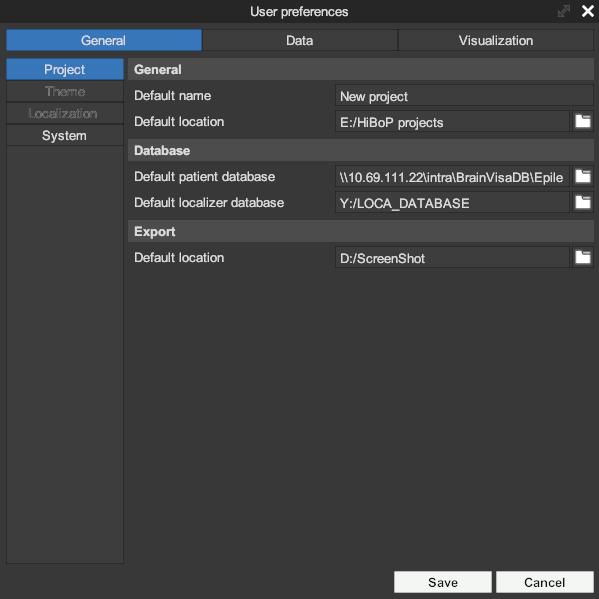
\includegraphics[scale=0.5]{Preferences.png}
\end{center}
\caption{\label{preferencesUI}User Preferences}
\end{figure}
\begin{itemize}
\item \textbf{General}
\begin{itemize}
\item \textbf{Project}
\begin{itemize}
\item \textbf{General}
\begin{itemize}
\item \textbf{Default name}: Default name for a new project
\item \textbf{Default location}: Default path to search for projects
\end{itemize}
\item \textbf{Database}
\begin{itemize}
\item \textbf{Default patient database}: Default path to the patient database
\item \textbf{Default localizer database}: Default path to functional data
\end{itemize}
\item \textbf{Export}
\begin{itemize}
\item \textbf{Default location}: Default path to save screenshots
\end{itemize}
\end{itemize}
\item \textbf{System}
\begin{itemize}
\item \textbf{Performance}
\begin{itemize}
\item \textbf{Enable multithreading}: Enable multithreading for calculation (e.g. EEG signal on the brain mesh)
\item \textbf{Memory cache limit}: Maximum amount of memory taken by HiBoP
\end{itemize}
\end{itemize}
\end{itemize}
\item \textbf{Data}
\begin{itemize}
\item \textbf{EEG}
\begin{itemize}
\item \textbf{Processing}
\begin{itemize}
\item \textbf{Averaging method}: Method to average the data (mean or median)
\item \textbf{Normalizing method}: The following formula is applied to each value $v$ $$v = \frac{v - \mu_{b}}{\sigma_{b}}$$ where $b$ is an array of the baseline values depending on this parameter, $\mu_b$ is their mean and $\sigma_b$ is their standard deviation
\end{itemize}
\end{itemize}
\item \textbf{Event}
\begin{itemize}
\item \textbf{Processing}
\begin{itemize}
\item \textbf{Position averaging method}: Method to average the position of the secondary events (mean or median)
\end{itemize}
\end{itemize}
\item \textbf{Anatomy}
\begin{itemize}
\item \textbf{Performances}
\begin{itemize}
\item \textbf{Enable mesh preloading}: Preload every meshes at the start of a visualization
\item \textbf{Enable MRI preloading}: Preload every MRIs at the start of a visualization
\item \textbf{Enable implantation preloading}: Preload every implantations at the start of a visualization
\end{itemize}
\item \textbf{Processing}
\begin{itemize}
\item \textbf{Enable site name correction}: Change the name of a certain patern of site names (for instance "xp4" becomes "X'4")
\end{itemize}
\end{itemize}
\end{itemize}
\item \textbf{Visualization}
\begin{itemize}
\item \textbf{3D}
\begin{itemize}
\item \textbf{EEG}
\begin{itemize}
\item \textbf{Enable automatic EEG update}: Triggers the update of the brain activity on the brain each time a parameter is changed in the visualization
\item \textbf{Site influence by distance}: Controls how a site influence its environment (constant amplitude, linear decrease or quadratic decrease)
\end{itemize}
\item \textbf{Single/Multi patient visualization}
\begin{itemize}
\item \textbf{Default selected MRI}: Select the MRI corresponding to this name when loading a new visualization, or the first in the list if the name does not match any
\item \textbf{Default selected mesh}: Select the mesh corresponding to this name when loading a new visualization, or the first in the list if the name does not match any
\item \textbf{Default selected implantation}: Select the implantation corresponding to this name when loading a new visualization, or the first in the list if the name does not match any
\end{itemize}
\end{itemize}
\item \textbf{Trial Matrix}
\begin{itemize}
\item \textbf{General}
\begin{itemize}
\item \textbf{Show whole protocol}: Display the matrices of all blocs of a protocol even if no column is set with some blocs of the protocol
\item \textbf{Enable trials synchronization}: Synchronize selected trials when comparing matrices of two sites
\end{itemize}
\item \textbf{Smoothing}
\begin{itemize}
\item \textbf{Enable trial smoothing}: Smoothes the trials of a matrix
\item \textbf{Number of intermediate values}: Number of values to be added between two real values during smoothing process
\end{itemize}
\item \textbf{Format}
\begin{itemize}
\item \textbf{Bloc format}: Changes how a bloc of the matrix is rendered (trials height in pixels, trial ratio or bloc ratio)
\end{itemize}
\end{itemize}
\item \textbf{Graph}
\begin{itemize}
\item \textbf{General}
\begin{itemize}
\item \textbf{Show curves of minimized columns}: Display all curves even if the corresponding column is minimized
\end{itemize}
\end{itemize}
\item \textbf{Cut}
\begin{itemize}
\item \textbf{Display}
\begin{itemize}
\item \textbf{Enable cut lines}: Display other cuts by lines on cut textures
\end{itemize}
\item \textbf{Performance}
\begin{itemize}
\item \textbf{Enable simplified mesh during cuts}: Change the currently used mesh to a simplified one to optimize the cutting process
\end{itemize}
\end{itemize}
\end{itemize}
\end{itemize}
\subsection{Project management}
\subsubsection{Creating, opening and saving a project}
\paragraph{} When creating a new project, you have to specify the name of your new project, the location where it will be saved, the location of the anatomical database and the location of the functional database (Figure \ref{newProjectUI}). The two last fields are optional.
\begin{figure}[H]
\begin{center}
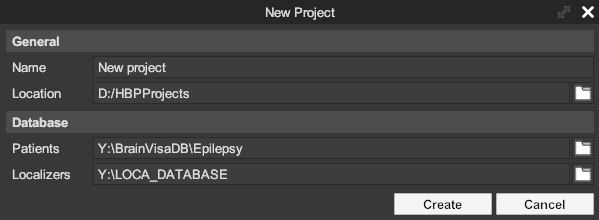
\includegraphics[scale=0.5]{NewProject.png}
\end{center}
\caption{\label{newProjectUI}Create a new project}
\end{figure}
\paragraph{} In order to open a previously created project (Figure \ref{openProjectUI}), you have to tell where your projects are located. Once these are loaded, you can either double click on the project you want to open or select the project and then click on Open. You can also sort projects using specific parameters.
\begin{figure}[H]
\begin{center}
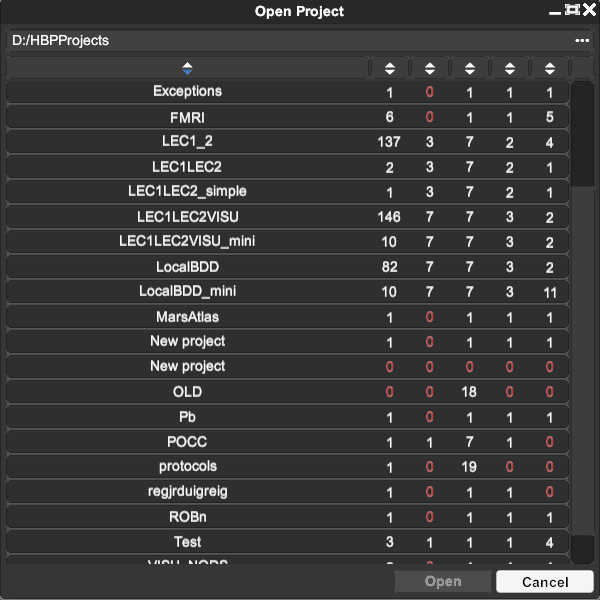
\includegraphics[scale=0.5]{OpenProject.png}
\end{center}
\caption{\label{openProjectUI}Open a project}
\end{figure}
\paragraph{} If you want to save a project to a different location or with a different name than when it was open, you can use the "Save as" menu (Figure \ref{saveProjectUI}).
\begin{figure}[H]
\begin{center}
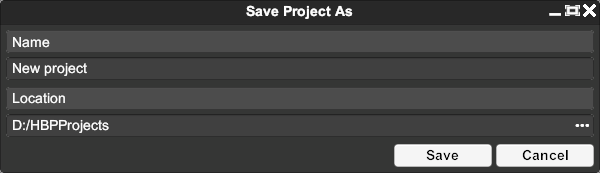
\includegraphics[scale=0.5]{SaveAs.png}
\end{center}
\caption{\label{saveProjectUI}Save a project as}
\end{figure}
\paragraph{} All of these menus are located in the File menu at the top of the screen.
\subsubsection{Patients management}
\paragraph{} To add patients to the opened project, you have to use the patients manager (Figure \ref{patientGestionUI}). The window has two panels: the left panel displays all available patients in the database (found in the folder you specify at the top of the window) whereas the right panel displays patients added to this project. For each patient, numbers indicate the status of their respective anatomical data (Meshes, MRIs, Implantations and Connectivities). To add or remove patients, you can either select them in any list and use the arrows to add or remove them, or you can create new patients from scratch using the "+" button in the center. In order for the anatomical database to be correctly loaded, you have to use a specific hierarchy described in appendix \ref{bddhierarchy}.
\begin{figure}[H]
\begin{center}
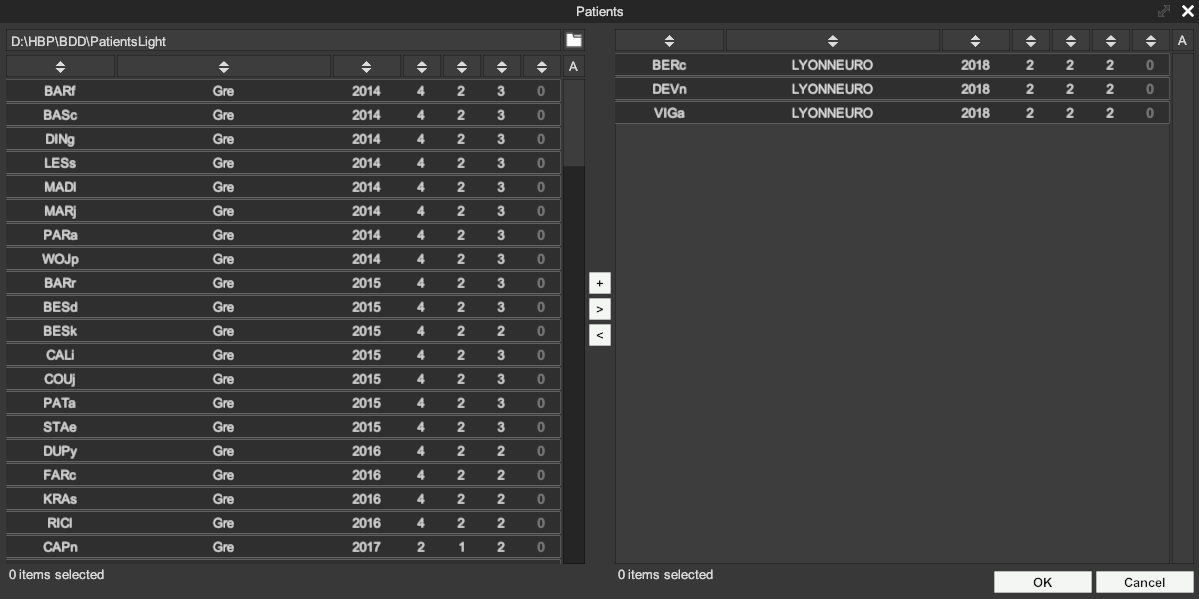
\includegraphics[scale=0.3]{PatientGestion.png}
\end{center}
\caption{\label{patientGestionUI}Patients manager}
\end{figure}
\paragraph{} To edit any loaded patient, you can double click\footnote{The process of double clicking an item to edit it is common to most windows of HiBoP} on it. This will open the patient modifier window (Figure \ref{patientModifierUI}) which will allow you to edit anything concerning the metadata or the anatomical data of this patient. You can navigate between anatomical data types using the tabs in the middle of the window.
\begin{figure}[H]
\begin{center}
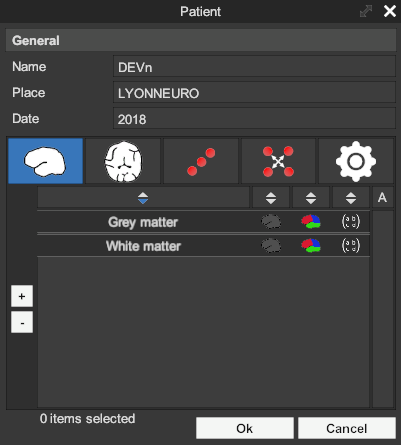
\includegraphics[scale=0.5]{PatientModifier.png}
\end{center}
\caption{\label{patientModifierUI}Patient modifier}
\end{figure}
\paragraph{} If you want to add a mesh, you can use the "+" button located to the left; if you want to edit a mesh, you can double click the mesh item, and this will open a mesh modifier window (Figure \ref{meshModifierUI}) which will allow you to edit the path to the GIfTI files or to the transformation file. Adding and editing other types of anatomical data is very similar.
\begin{figure}[H]
\begin{center}
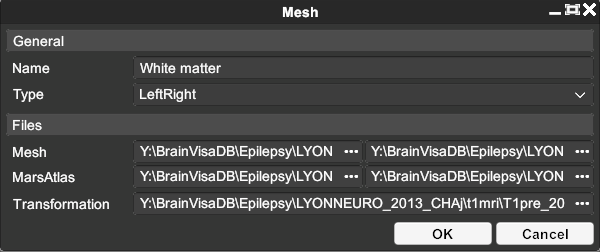
\includegraphics[scale=0.5]{MeshModifier.png}
\end{center}
\caption{\label{meshModifierUI}Mesh modifier}
\end{figure}
\paragraph{} As stated in section \ref{data}, you can also create groups of patients to add them more easily to the visualizations. This is done through the groups manager window (Figure \ref{groupGestionUI}). To create a new group, use the "+" button on the left. To remove existing groups, select the group(s) you want to remove, and use the "-" button on the left\footnote{The process of using "+" button to add and "-" button to remove is common to most windows of HiBoP}. Adding and removing patients from a group is very similar to the patients manager window (Figure \ref{groupModifierUI}).
\begin{figure}[H]
\begin{center}
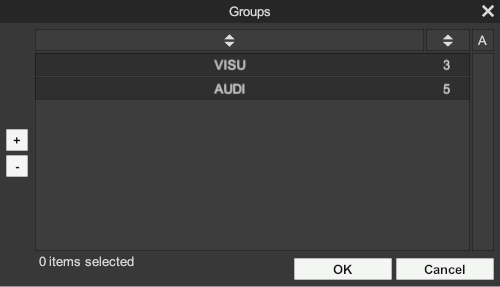
\includegraphics[scale=0.5]{GroupGestion.png}
\end{center}
\caption{\label{groupGestionUI}Groups manager}
\end{figure}
\begin{figure}[H]
\begin{center}
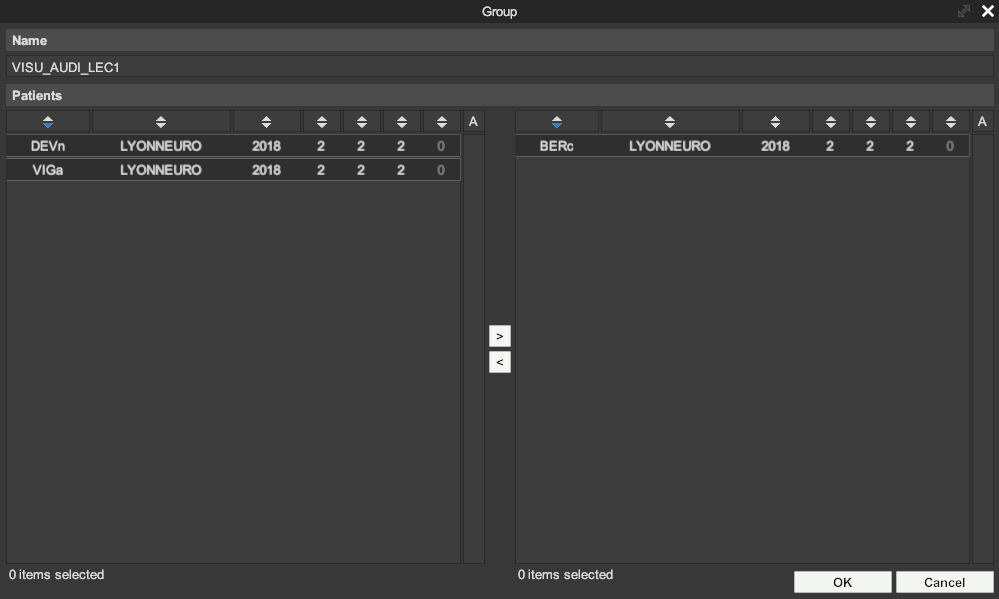
\includegraphics[scale=0.3]{GroupModifier.png}
\end{center}
\caption{\label{groupModifierUI}Group modifier}
\end{figure}
\subsubsection{Data management}
\paragraph{} First thing to do concerning data management is to create a protocol that will epoch the iEEG data. You can do that using the protocol manager window (Figure \ref{protocolGestionUI}). You can also import an existing .prov file to the project by using the "Import..." button on the bottom.
\begin{figure}[H]
\begin{center}
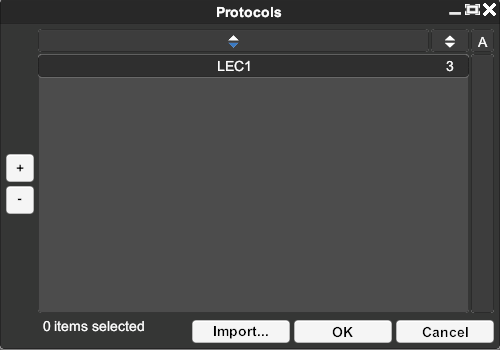
\includegraphics[scale=0.5]{ProtocolGestion.png}
\end{center}
\caption{\label{protocolGestionUI}Protocols manager}
\end{figure}
\paragraph{} Editing a protocol consists of defining the blocs for this protocol. This is done with the protocol modifier window (Figure \ref{protocolModifierUI}). To create a new bloc, click on an empty box. To edit a bloc, double click on an existing bloc.
\begin{figure}[H]
\begin{center}
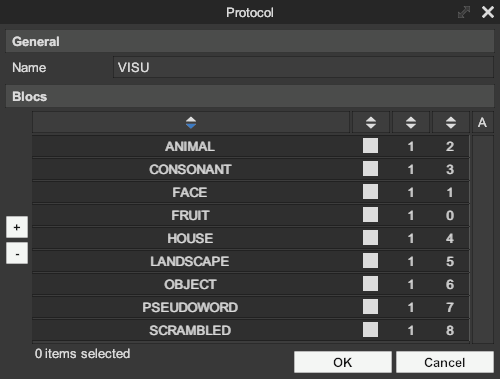
\includegraphics[scale=0.4]{ProtocolModifier.png}
\end{center}
\caption{\label{protocolModifierUI}Protocol modifier}
\end{figure}
\paragraph{} A bloc can be edited with the bloc modifier window (Figure \ref{blocModifierUI}). There you can specify the name, the sorting method, and define the subblocs using the subbloc modifier window (Figure \ref{subBlocModifierUI}). There, you can edit the name, the order, the type (main or secondary), the window, the baseline window, the events and the iconic scenario of the subbloc.
\begin{figure}[H]
\begin{center}
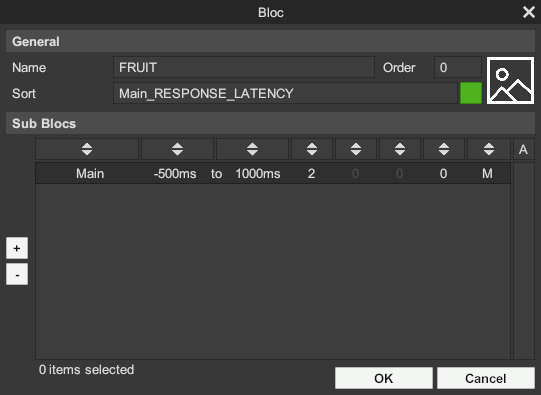
\includegraphics[scale=0.5]{BlocModifier.png}
\end{center}
\caption{\label{blocModifierUI}Bloc modifier}
\end{figure}
\begin{figure}[H]
\begin{center}
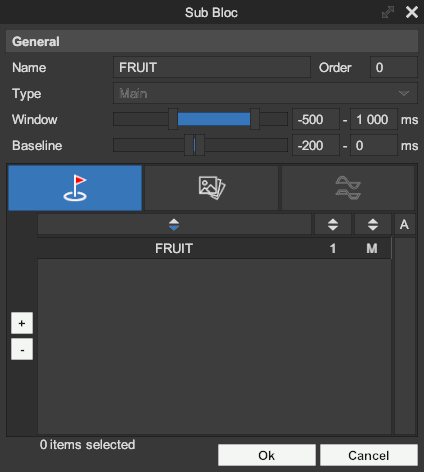
\includegraphics[scale=0.5]{SubBlocModifier.png}
\end{center}
\caption{\label{subBlocModifierUI}SubBloc modifier}
\end{figure}
\paragraph{} When your protocols are correctly defined, you are ready to create your datasets. This will be done using the datasets manager window (Figure \ref{datasetGestionUI}).
\begin{figure}[H]
\begin{center}
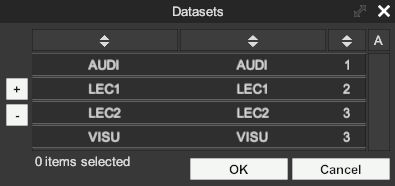
\includegraphics[scale=0.5]{DatasetGestion.png}
\end{center}
\caption{\label{datasetGestionUI}Datasets manager}
\end{figure}
\paragraph{} For a given dataset, you need to give it a name and assign a protocol. All the data included in this dataset will be epoched regarding the chosen protocol. With the dataset modifier window (Figure \ref{datasetModifierUI}), you can add and edit data information. Each data information has a little colored box which indicates the status of the data information : red means it is unsuable, whereas green means you can visualize it. You can click on this box to have more information about the data information.
\begin{figure}[H]
\begin{center}
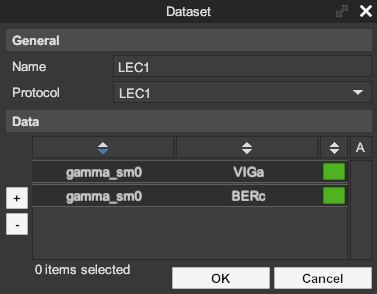
\includegraphics[scale=0.5]{DatasetModifier.png}
\end{center}
\caption{\label{datasetModifierUI}Dataset modifier}
\end{figure}
\paragraph{} A data information has a name and is linked to a patient. A single dataset can not have two data information with the same pair [name, patient]. Data are identified by their names, so if you want to visualize data of several patients in the same column, you have to give them the same name (since their respective patient will be different, the pairs [name, patient] will be different). Then, you have to fill in the paths to the functional data files (.eeg and .pos). The label in front of the EEG file path corresponds to the label of the data you want to extract from the EEG file (usually, it is "EEG data"). You can also change how this particular data will be normalized (this overwrites the global parameter for normalization).
\begin{figure}[H]
\begin{center}
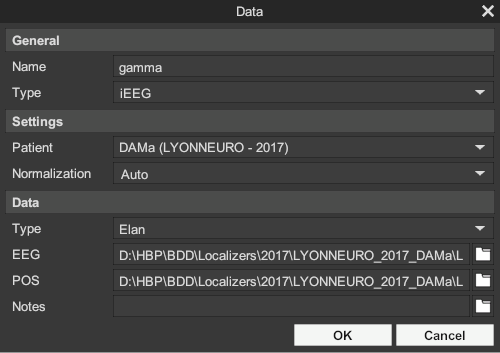
\includegraphics[scale=0.5]{DataInfoModifier.png}
\end{center}
\caption{\label{dataInfoModifierUI}Data information modifier}
\end{figure}
\subsubsection{Visualizations management}
\paragraph{} When everything is set up, you can create visualizations. This is done using the visualization manager window (Figure \ref{visuGestionUI}).
\begin{figure}[H]
\begin{center}
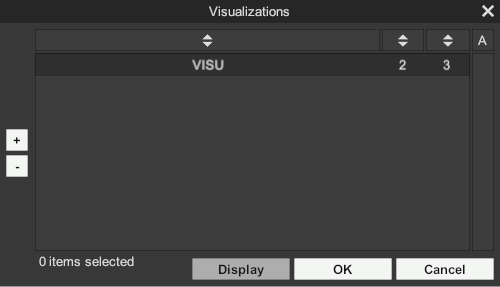
\includegraphics[scale=0.5]{VisualizationGestion.png}
\end{center}
\caption{\label{visuGestionUI}Visualizations manager}
\end{figure}
\paragraph{} A visualization has a name, patients and columns. To edit all of this information, you can use the visualization modifier window (Figure \ref{visuModifierUI}). To add patients to the visualization, use the arrows (same process than adding patients to the project). To add a column, click on the "+" button under the "Columns" panel. You can then edit the column by setting the name, the type (anatomy only or iEEG), the protocol, the bloc, the dataset and the data name to be used in this column. Do not forget that if multiple patients are added to the visualization, they must have at least one data information with the same name.
\begin{figure}[H]
\begin{center}
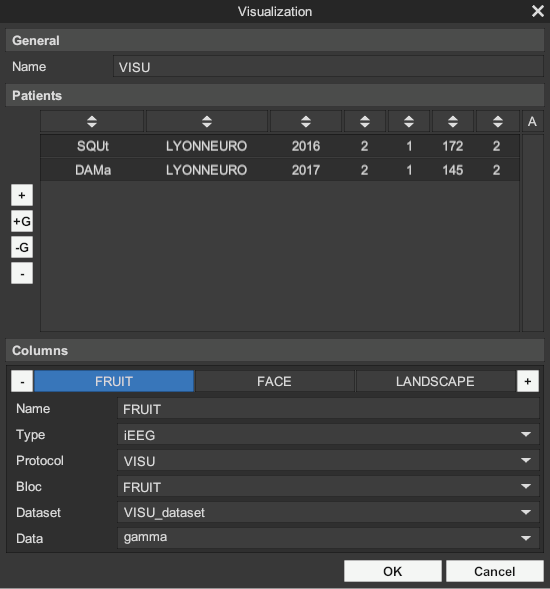
\includegraphics[scale=0.3]{VisualizationModifier.png}
\end{center}
\caption{\label{visuModifierUI}Visualization modifier}
\end{figure}
\paragraph{} Once your visualizations are ready to be displayed, you can select them and click the "Display" button.
\subsection{3D Visualization}
\paragraph{}
\begin{figure}[H]
\begin{center}
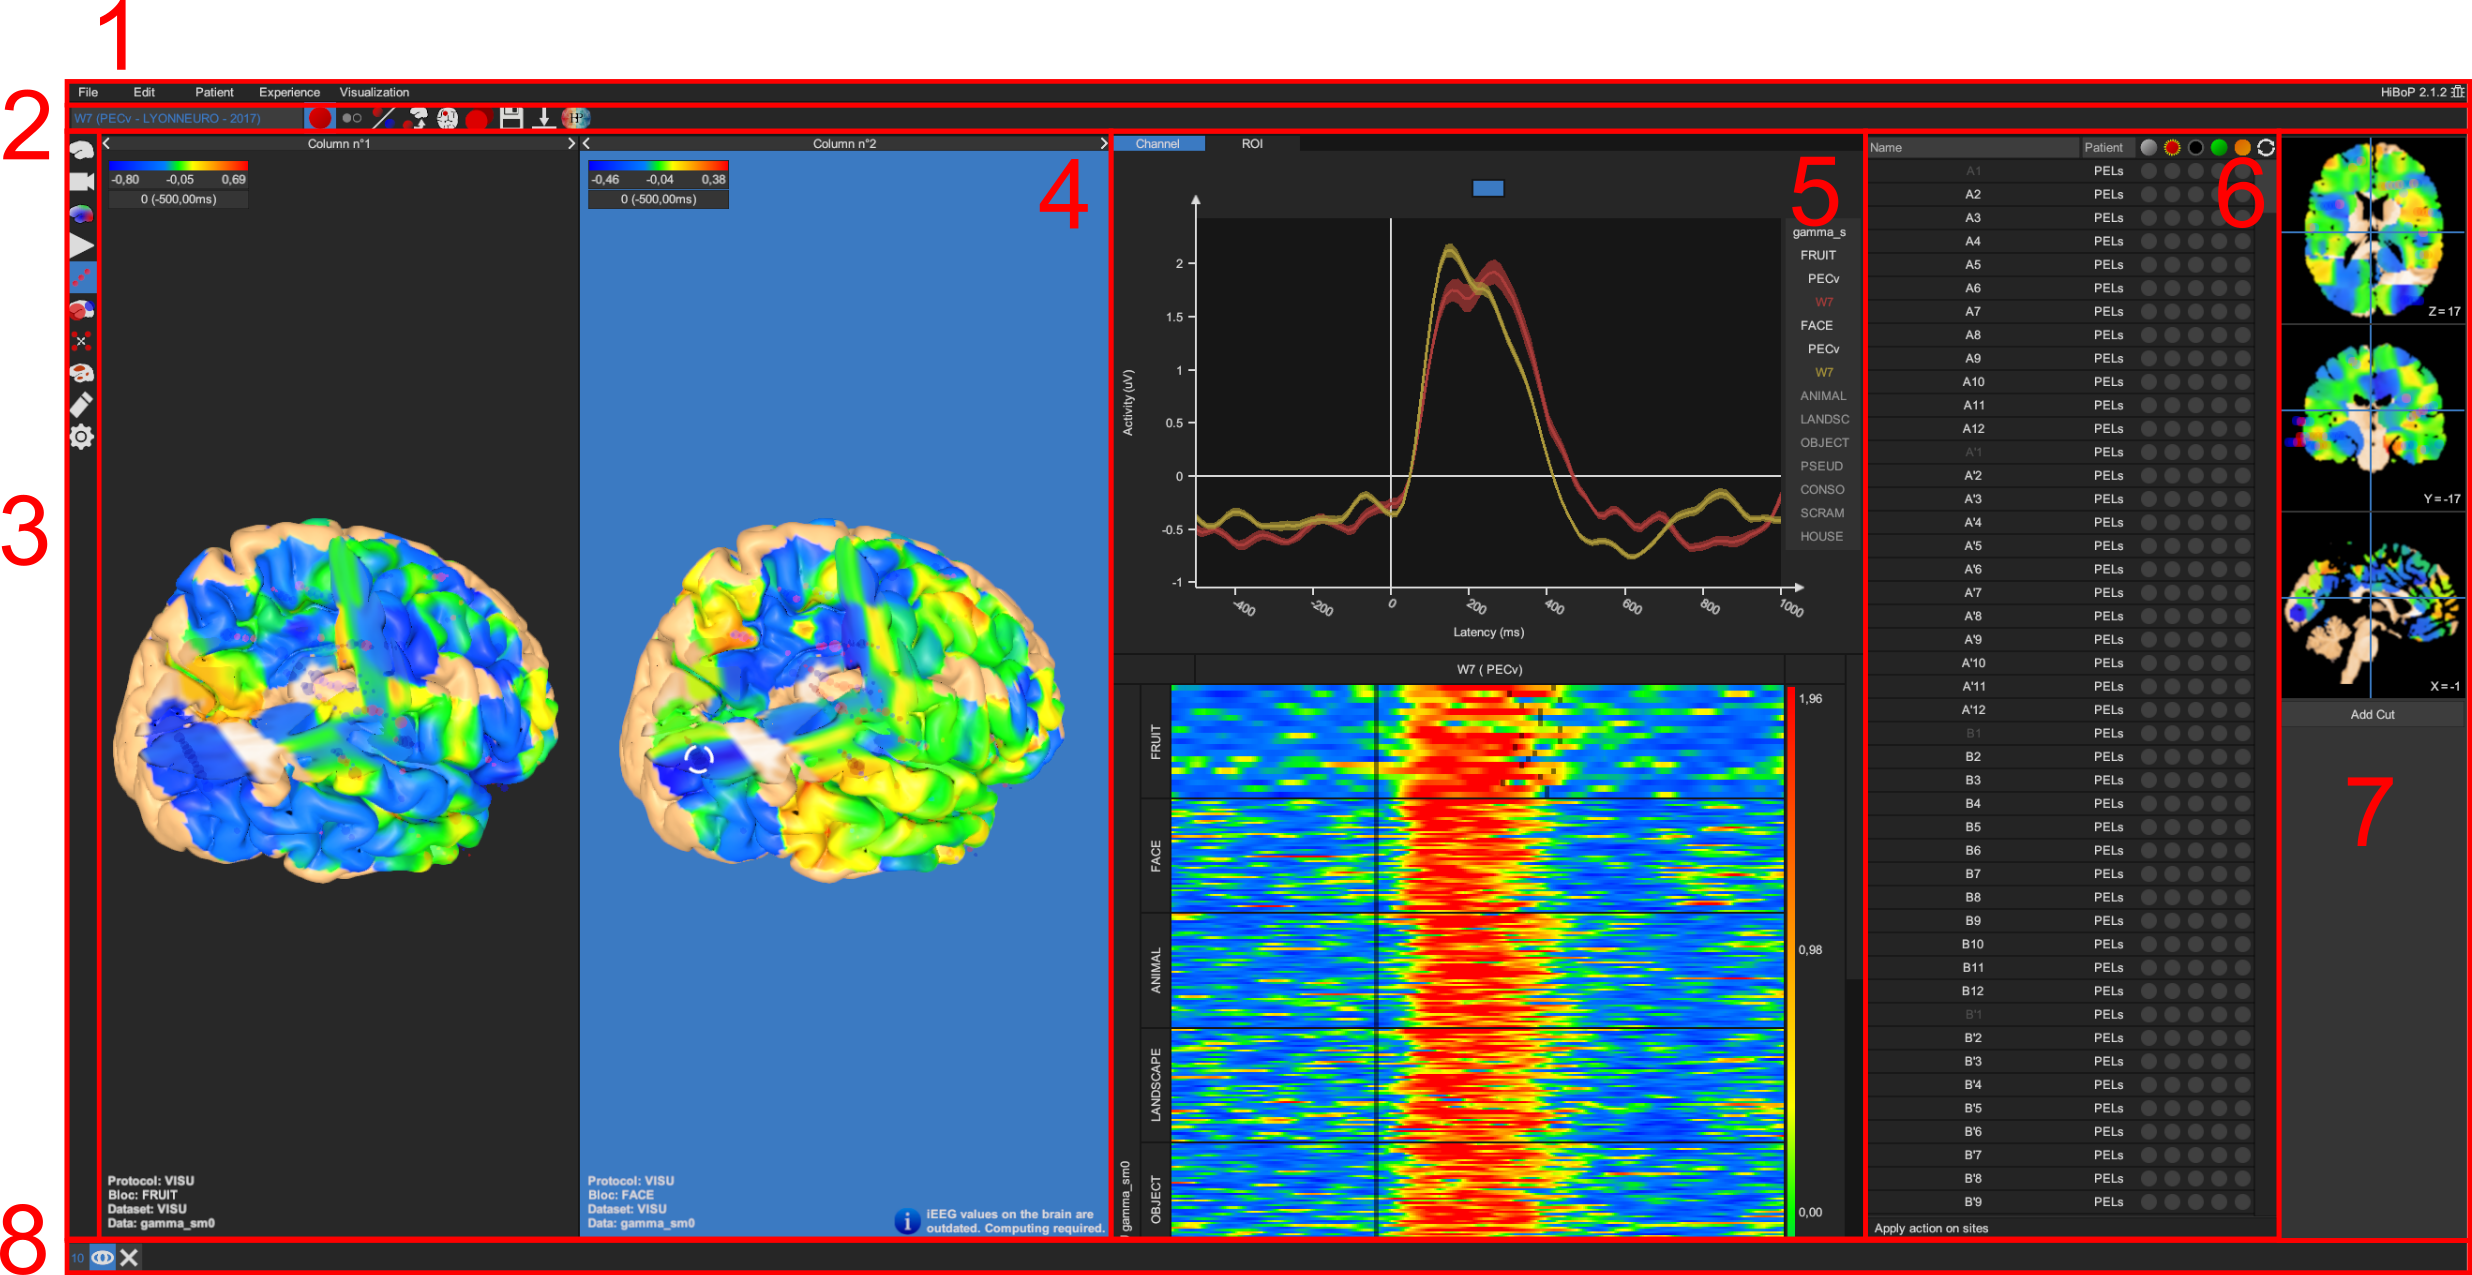
\includegraphics[scale=0.7]{GlobalUI.png}
\end{center}
\caption{\label{globalUI}HiBoP user interface}
\end{figure}
\paragraph{} The main user interface of HiBoP can be decomposed as follow (Figure \ref{globalUI}) :
\begin{itemize}
\item \textbf{1} - Main menu (data management, see section \ref{UI} for more information)
\item \textbf{2} - Toolbar (used to do actions on the 3D scene, more information in later sections)
\item \textbf{3} - Toolbar selector (to select which toolbar you want to use)
\item \textbf{4} - 3D visualization (main visualization window)
\item \textbf{5} - Graphs and trial matrices (precise information of iEEG data, see section \ref{graphs})
\item \textbf{6} - Cut panel (manage cuts, see section \ref{cuts})
\item \textbf{7} - Opened visualizations (used to minimize or close opened visualizations)
\end{itemize}
\paragraph{} Elements in parts 4, 5 and 6 can be resized using the black handlers betweens them. Columns of the 3D vizualisations can be moved by drag and dropping their labels at the top of the column. You can interact with the scene in many ways :
\begin{itemize}
\item Left click on a view to select the corresponding view / column / scene or left click on a site / on a ROI to select it.
\item Right click and drag to rotate the brain surface
\item Middle click and drag to translate the brain surface
\item Use the scroll wheel to control the zoom
\item Drag and drop the name of a column to swap it with another column or to insert it between two columns
\end{itemize}
\paragraph{} The left panel allows you to change between toolbars. Each toolbar has its own functions, which will be explained in more details in later sections.
\newline
\begin{minipage}{0.2\textwidth}
\begin{figure}[H]
\begin{center}

\includegraphics[scale=0.75]{ToolbarSelector.png}
\end{center}
\end{figure}
\end{minipage}
\begin{minipage}{0.5\textwidth}
\begin{itemize}
\item Scene settings
\item Display settings
\item iEEG settings
\item Timeline
\item Sites
\item Regions of Interest
\item CCEP
\item fMRI
\item Triangle eraser
\item Configuration
\end{itemize}
\end{minipage}
\subsubsection{Cuts}\label{cuts}
\paragraph{} Before getting into the toolbars, let's talk about cuts. Indeed, HiBoP allows you to cut the 3D mesh (using the MRI to fill the cut plane) with the right panel. To add a cut, click on the "Add cut" button. You can change parameters on the cut after clicking on it to open the parameters panel (Figure \ref{cut}). You can change its orientation (Axial, Coronal, Sagital or Custom), you can flip it (Axial, Coronal and Sagital) or set up a custom normal (Custom), you can change the position of the cut using the slider or the "+" and "-" buttons for more precision. To delete a cut, open the parameters panel and click on the little cross on the top-right of the cut.
\begin{figure}[H]
\begin{center}
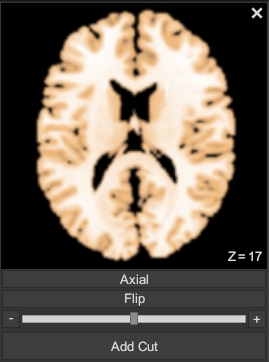
\includegraphics[scale=0.5]{Cut.png}
\end{center}
\caption{\label{cut}Cut parameters panel}
\end{figure}
\subsubsection{Sites list}\label{sitesList}
\paragraph{} A list of all the sites of the scene is available in the corresponding panel (Figure \ref{sitesListPanel}). This list displays all sites found in the PTS files and their states, even if they do not have a corresponding channel in an EEG file (sites with no value will have their name in grey and will not be selectable). You can filter the sites by name, patient name and states.  Available states are :
\begin{itemize}
\item Excluded : an excluded site is not in the iEEG computations, but it remains visible in the scene
\item Highlighted : a highlighted site appears without transparency in the scene
\item Marked : a marked site appears in green when the iEEG are not computed (the behaviour is the same as an included site)
\item Blacklisted : a blacklisted site is barely visible and not included in any calculation
\item Suspicious : a suspicious site appears orange in the scene
\end{itemize}
\begin{figure}[H]
\begin{center}
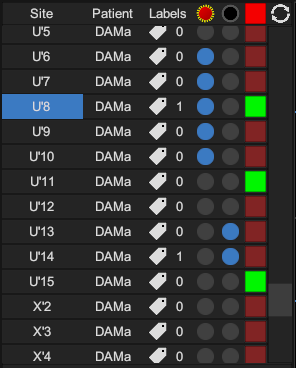
\includegraphics[scale=0.5]{SitesList.png}
\end{center}
\caption{\label{sitesListPanel}Sites list panel}
\end{figure}
\paragraph{} This panel also allows you to change the states of some sites directly. You can achieve this in 3 different ways :
\begin{itemize}
\item You can click on the dots to set or unset the state of a specific site in the list.
\item You can use the submenu "Apply state on sites". There, you can filter sites using specific conditions concerning their current states, their location, information about them or their EEG signal, and apply states by selecting the icons of the states and clicking on the apply button. This process correspond to the "Basic" way of setting multiple states at once (Figure \ref{basicStates}).
\item The "Advanced" way can be accessed through the Advanced tab of the aforementioned submenu. While the Basic tab can only filter sites with a global AND between all conditions (which means that all conditions must be fulfilled for a site in order to apply the states), the Advanced tab can be used to create more complex conditions. You can click on the "?" icon to have a detailed description on how it works, alongside examples.
\end{itemize}
\begin{figure}[H]
\begin{center}
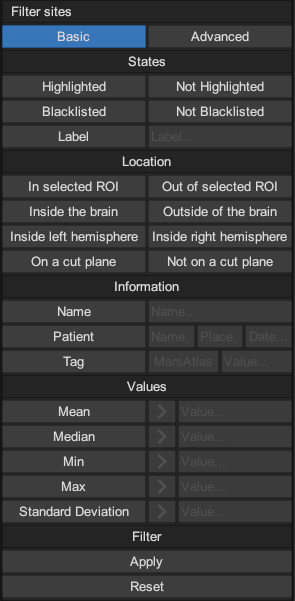
\includegraphics[scale=0.5]{BasicStates.png}
\end{center}
\caption{\label{basicStates}Apply state on sites submenu (in this example, sites that are in the selected ROI (Section \ref{roi}) and which values have a mean above 110 will be marked suspicious)}
\end{figure}
\paragraph{} The following sections will explain the different functionalities of each toolbar.
\subsubsection{Scene settings}
\begin{figure}[H]
\begin{center}
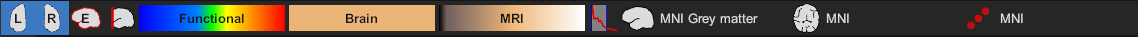
\includegraphics[scale=0.45]{SceneSettings.png}
\end{center}
\end{figure}
\begin{itemize}
\item Display both parts, only the left part or only the right part of the selected mesh (only works for left-right meshes).
\item Display mars atlas on the mesh (only works if the mars atlas field of the mesh is valid).
\item Display the edges of the mesh.
\item Switch between the soft cut mode (keep everything behind a cut) and the hard cut mode (cut everything in front of a cut).
\item Change the colormap of the iEEG values.
\item Change the color of the brain.
\item Change the color of the cuts.
\item Change the threshold of the MRI values (contrast). Use the sliders to change these values.
\item Change the mesh (MNI meshes are available no matter the number of patients, the patient meshes are only available if the patient is alone in the visualization).
\item Change the MRI (patient MRIs are only available if the patient is alone in the visualization).
\item Change the implantation (an implantation is available only if each patient of the visualization has an implantation with the same name)
\end{itemize}
\subsubsection{Display settings}
\begin{figure}[H]
\begin{center}

\includegraphics[scale=0.45]{DisplaySettings.png}
\end{center}
\end{figure}
\begin{itemize}
\item Add or remove a view (maximum 5 views).
\item Set up standard views (3 views with 3 different points of view).
\item Reset the camera position of the selected view.
\item Reset the size of the views (if resized using the handlers).
\item Automatic rotation of the brain (you can set the rotation speed with the slider).
\item Change the camera behaviour (T = trackball camera, O = orbital camera).
\item Take a raw screenshot of the scene which will be saved in the default export directory (set in user preferences).
\item Save the scene as files in a directory named after the name of the visualization in the default export directory (one image per opened view, one image per cut, one image and one svg for the graph, one image for the trial matrices, one csv for each curve containing the values).
\end{itemize}
\subsubsection{iEEG settings}
\begin{figure}[H]
\begin{center}

\includegraphics[scale=0.45]{iEEGSettings.png}
\end{center}
\end{figure}
\begin{itemize}
\item Trigger global mode (any changes will be applied to all columns)
\item Change the size of the sites
\item Change the size of the influence sphere of the sites (to compute the iEEG on the brain surface)
\item Change the transparency of the iEEG value on the brain surface
\item Change the threshold values for the iEEG (anything less than the minimum value will be of the same color as the minimum value, the same apply for the maximum value; the rest of the values will increase linearly from minimum to middle and then increase linearly from middle to maximum). You can change these values by either using the sliders or editing the numbers in the boxes. There are 2 modes : the symmetric mode allows you to set the middle value and the amplitude, whereas the asymmetric mode allows you to set each value independently.
\item Compute the iEEG values on the brain surface or clean the brain.
\end{itemize}
\subsubsection{Timeline}
\begin{figure}[H]
\begin{center}

\includegraphics[scale=0.45]{Timeline.png}
\end{center}
\end{figure}
\begin{itemize}
\item Trigger global mode (any changes will be applied to all columns).
\item Make the timeline play automatically.
\item Increase the current timeline ID by a specific amount of samples (this also controls the speed of the play, X samples will be played each second).
\item Loop the timeline (when playing automatically).
\item Slider to control the timeline precisely; the red mark indicates the main event, the blue marks indicates the secondary events (as defined in the .prov file).
\end{itemize}
\subsubsection{Sites}
\begin{figure}[H]
\begin{center}
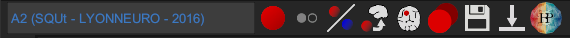
\includegraphics[scale=0.45]{Sites.png}
\end{center}
\end{figure}
\begin{itemize}
\item Selected site name.
\item Display all sites in the scene.
\item Hide blacklisted sites.
\item Compare two sites : select a site, click on this button, then select another site to compare them.
\item Load the single patient scene corresponding to the patient whose site is selected.
\item Cut the brain mesh around the select site.
\item Copy the states of the sites of the selected column to every other columns.
\item Save the states of the sites in a .csv file.
\item Load a .csv file with the states of the sites to the selected column.
\item Open the HBP Interactive Viewer centered around the selected site.
\end{itemize}
\subsubsection{Regions of Interest}\label{roi}
\paragraph{} Regions of Interest (ROI) are useful if you only want to study a small group of sites. They are composed of multiple spheres with different positions and radiuses. If the option "Show All Sites" of the sites toolbar is not enabled, only the sites of the selected ROI will be included in the iEEG computations on the brain. A curve will also be generated for the selected ROI of each column (section \ref{graphs}).
\begin{figure}[H]
\begin{center}
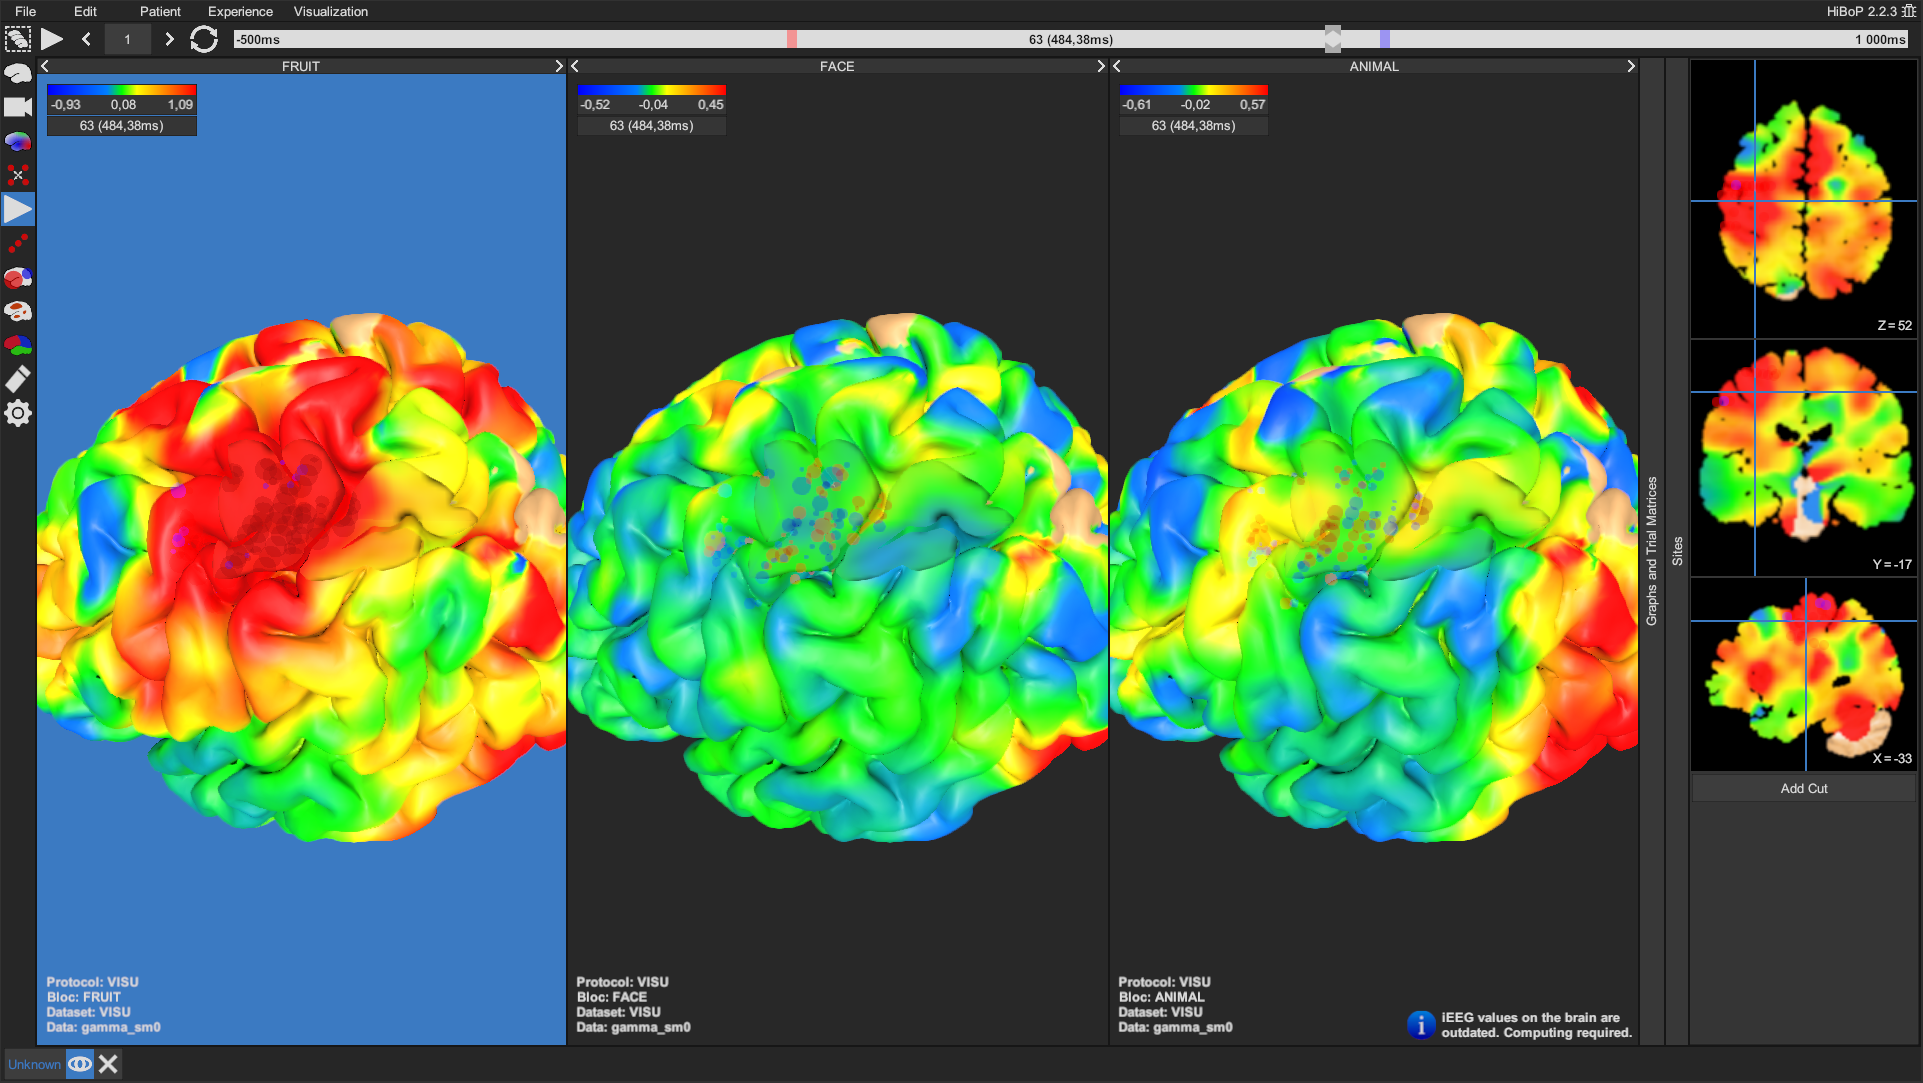
\includegraphics[scale=0.45]{ROI.png}
\end{center}
\end{figure}
\begin{itemize}
\item Add a new ROI in the selected column.
\item Select a ROI for the selected column.
\item Change the name of the selected ROI.
\item Remove the selected ROI.
\item Select a sphere of the ROI.
\item Delete the selected ROI.
\item Copy the selected ROI to other columns.
\item Save the selected ROI to a .roi file.
\item Load a .roi file to the selected column.
\item Export information about each site in the selected ROI (.csv file).
\end{itemize}
\paragraph{} After adding a ROI to the selected column, you can left click on the mesh to add spheres to this ROI. You can select a sphere using either the toolbar or by left clicking on it. You can change the position of the selected sphere by draging and droping it and its size using the scroll wheel.
\subsubsection{CCEP}
\paragraph{} This toolbar will allow you to enable CCEP mode (which will disable iEEG mode) and choose from the Connectivity files which one you want to display. To select a source, simply select the site you want as source.
\subsubsection{fMRI}
\begin{figure}[H]
\begin{center}

\includegraphics[scale=0.45]{fMRI.png}
\end{center}
\end{figure}
\begin{itemize}
\item Add or remove a fMRI to the anatomic MRI. If iEEG values are computed, the fMRI will not be displayed.
\item Change the threshold values of the fMRI.
\item Change the transparency of the fMRI.
\end{itemize}
\subsubsection{Triangle eraser}
\begin{figure}[H]
\begin{center}

\includegraphics[scale=0.45]{TriEraser.png}
\end{center}
\end{figure}
\begin{itemize}
\item Reset the triangle eraser.
\item Choose how you want to erase triangles (one triangle, cylinder, zone). To erase triangles, left click on the mesh where you want to erase them.
\item Expand the erased zone.
\item Invert the erased zone.
\item Revert last action.
\end{itemize}
\subsubsection{Configuration}
\paragraph{} This toolbar allow you to save, load or reset the configuration of the selected scene. Beware, saving the configuration will just save it to the loaded visualization: to write the changes in the corresponding file, you still have to save the whole project.
\subsection{Graphs and Trial Matrices}\label{graphs}
\paragraph{} The middle panel allows you to examine more precise information about the iEEG data of specific sites. You can open it using the handlers or if it is closed, it will automatically open once you select a site.
\subsubsection{Graphs}
\begin{figure}[H]
\begin{center}
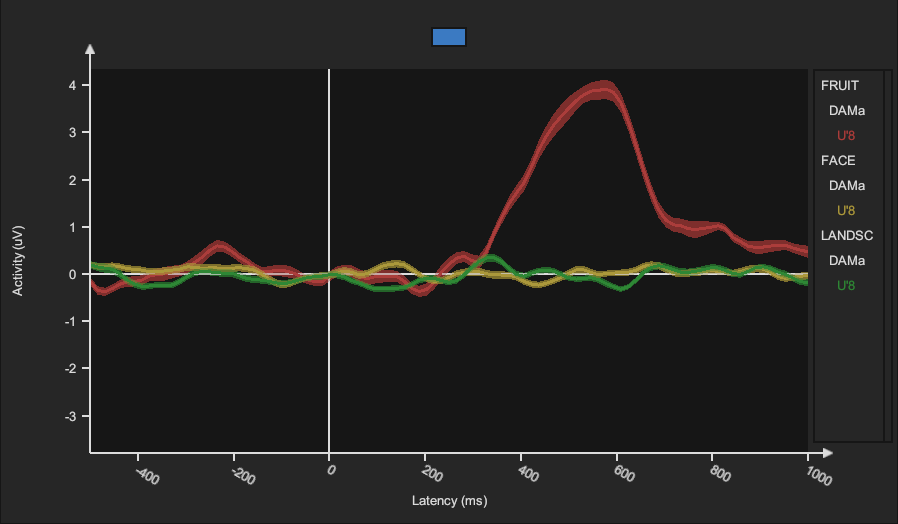
\includegraphics[scale=0.35]{Graph.png}
\end{center}
\caption{\label{graph}Graph for a protocol and two blocs (site D4 and ROI)}
\end{figure}
\paragraph{} Curves are generated for each column (or not minimized columns, depending on the chosen preferences) :
\begin{itemize}
\item One curve for the last selected site (the column in which the site has been selected does not matter)
\item One curve for the compared site if you are comparing two sites using the "Compare Site" tool in the site toolbar
\item One curve for the ROI if it exists. The ROI is considered as a single site which has the combined activity of all sites (excluding excluded or blacklisted sites) within it.
\end{itemize}
\paragraph{} An example of graph can be found at Figure \ref{graph}. A curve is the mean or median (depending on global preferences) of the iEEG activity of a site. The shapes around the single site curves correspond to the standard error of the mean (SEM). You can interact with the graph in order to get the most of it :
\begin{itemize}
\item You can hover a point with your mouse to see precise coordinates of this point.
\item You can zoom in and out using the mouse wheel and left click and drag to move the graph.
\item You can left click on an axis to precisely edit the viewport of the curve. This small window also has an "Auto" button; this functionality adapts the viewport so you can see every points of each curve.
\item You can hide a curve by left clicking on the corresponding item in the legend.
\end{itemize}
\subsubsection{Trial matrices}
\begin{figure}[H]
\begin{center}
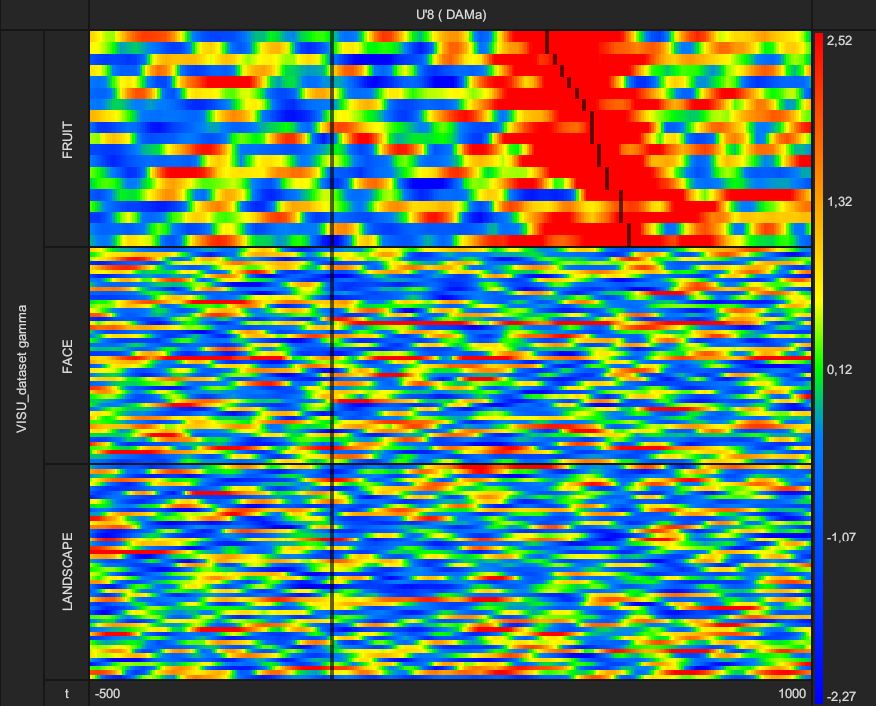
\includegraphics[scale=0.35]{TrialMatrix.png}
\end{center}
\caption{\label{trialMatrix}Trial matrix of a site}
\end{figure}
\paragraph{} Trial matrices are usefull to inspect iEEG activity of a site trial by trial. Trials are sorted according to the sorting method of a protocol bloc. You can change the color scale by clicking on it (same process as changing the viewport of the graph). Again, you can hover the matrix to get precise information about the hovered section (like in graphs). You can also select specific trials; only the selected trials will be taken into account when computing the values of the corresponding curve. To select trials, you can :
\begin{itemize}
\item Select a single trial by left clicking on it
\item Select multiple trials by either shift left clicking on the trials you want to select, or by pressing the left click button dragging the mouse and releasing the button.
\item Move the selection with the scroll wheel
\end{itemize}
\appendix
\section{HiBoP Database Manager}\label{bddmanager}
\paragraph{} The HiBoP Database Manager (DB Manager) can be used to manage the anatomical and functional databases (as long as they respect the hierarchy described in appendix \ref{bddhierarchy}), create HiBoP projects using huge amounts of data in no time or convert the databases to the Brain Imaging Data Structure (BIDS) format\footnote{More information about BIDS can be found at http://bids.neuroimaging.io/}. The main window (Figure \ref{dbManagerMain}) of the DB Manager has two main columns. The left column allows you to select patients to visualize their anatomical data, the right column is for functional data.
\begin{figure}[H]
\begin{center}
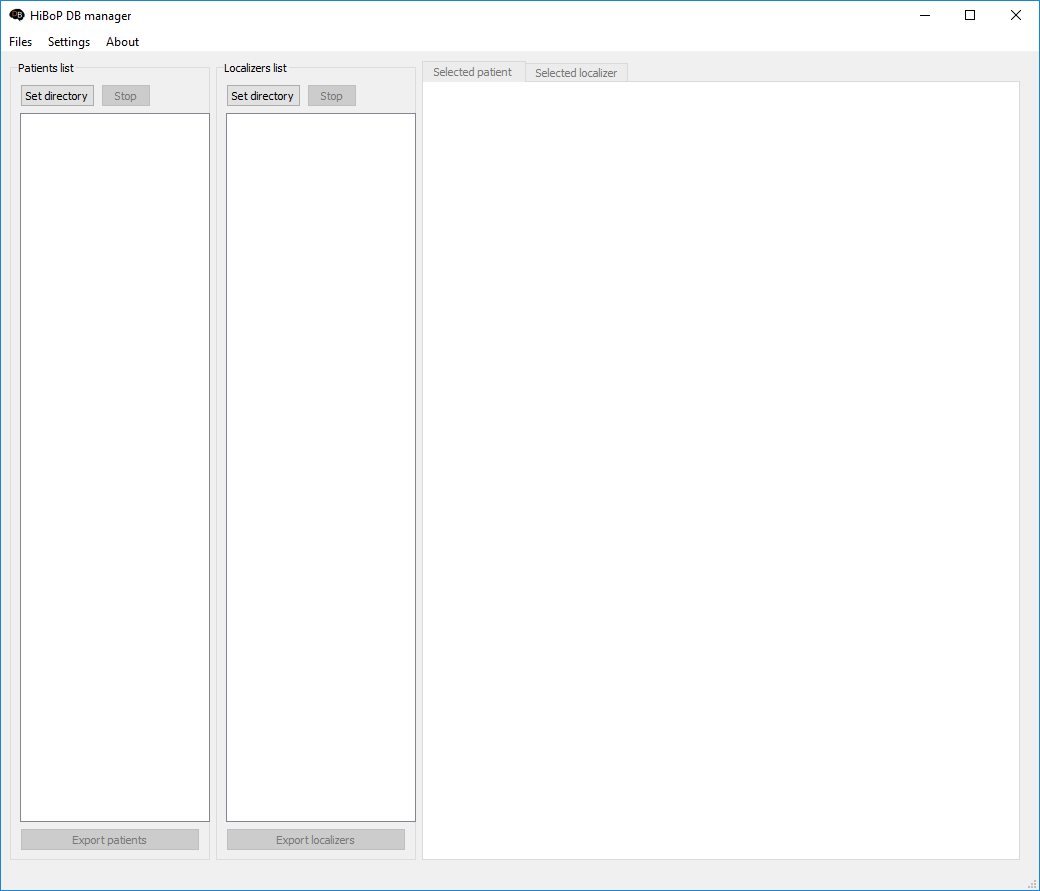
\includegraphics[scale=0.3]{DBManagerMain.png}
\end{center}
\caption{\label{dbManagerMain}Main window of the DB Manager}
\end{figure}
\subsection{Anatomical data}
\paragraph{} Click « Set Directory » in the first column to select the folder containing the anatomical database. After choosing a folder, patients found within that database will appear in the first column. Selecting one patient will display in the middle panel (Figure \ref{dbManagerPatient}) a list of files types and their status (present in green or absent in red). Some of the files can be visualized or opened directly from that interface. The display allows the user to quickly browse through patients and identify missing files.
\begin{figure}[H]
\begin{center}
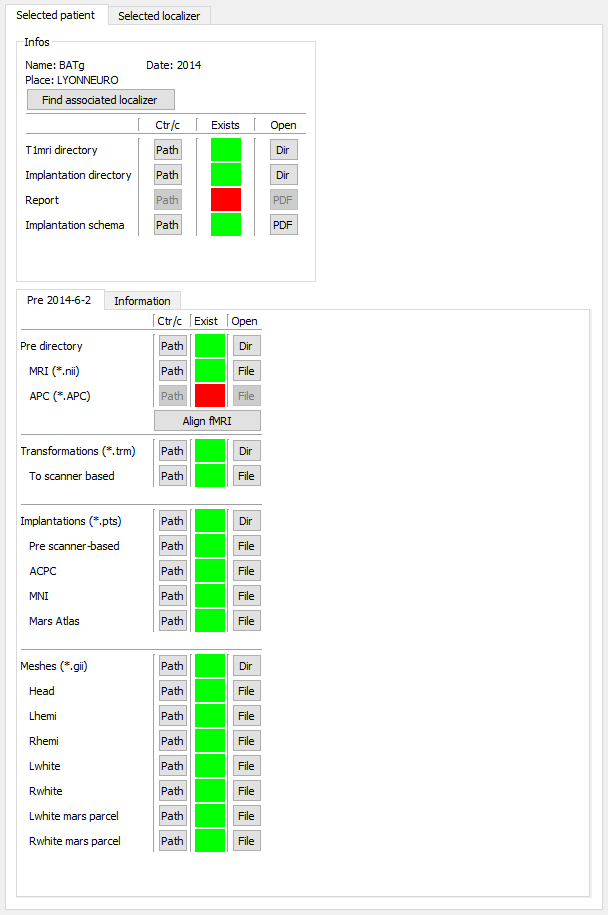
\includegraphics[scale=0.5]{DBManagerPatient.png}
\end{center}
\caption{\label{dbManagerPatient}Patient panel}
\end{figure}
\subsection{Functional data}
\paragraph{} Click « Set Directory » in the second column to select the folder containing the functional database. Once loaded, the database can be inspected patient by patient in a way similar to anatomical data (Figure \ref{dbManagerLoca}). Missing files can be quickly identified this way.
\begin{figure}[H]
\begin{center}
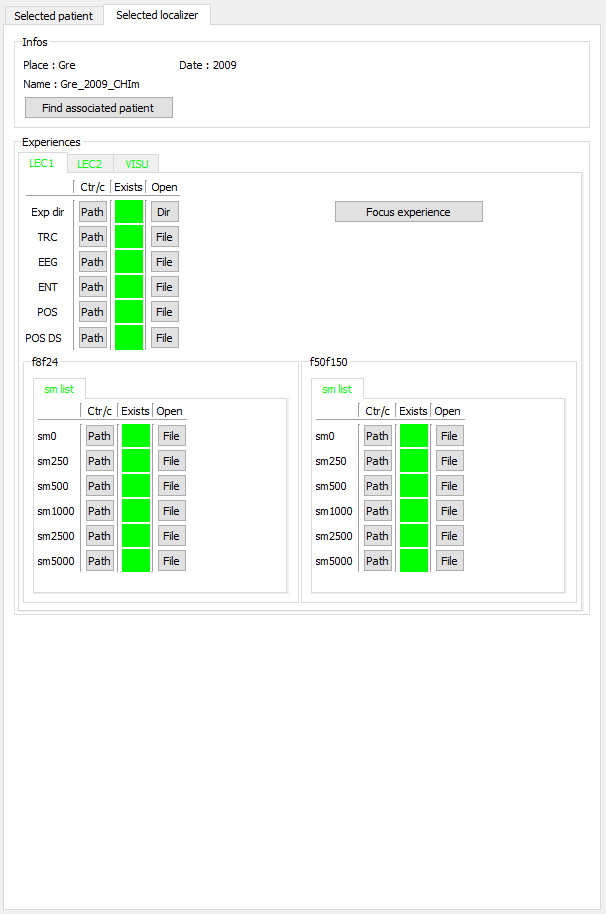
\includegraphics[scale=0.5]{DBManagerLoca.png}
\end{center}
\caption{\label{dbManagerLoca}Localizer (iEEG data) panel}
\end{figure}
\subsection{Exporting data}
\paragraph{} A panel in the right part (Figure \ref{dbManagerFilters}) of the window allows the user to filter patients. By checking boxes, you can quickly identify patients matching certain criteria (e.g. all patients with task LEC2, with gamma envelopes and anatomical MRIs).
\begin{figure}[H]
\begin{center}
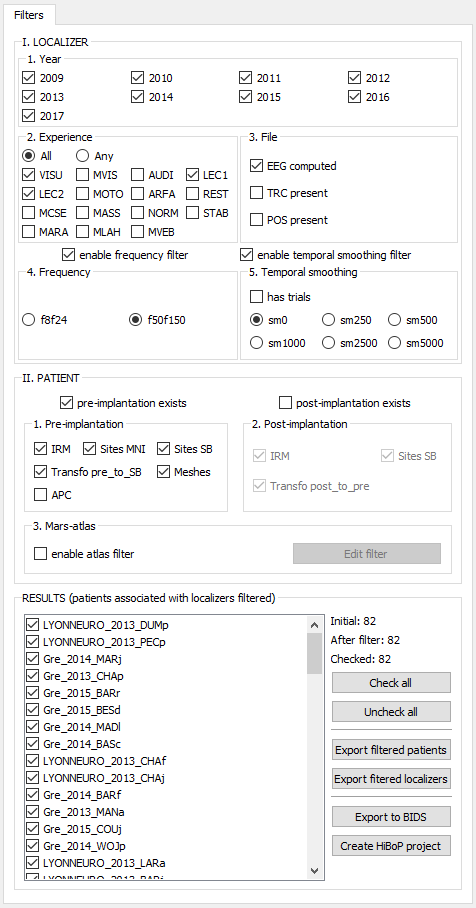
\includegraphics[scale=0.5]{DBManagerFilters.png}
\end{center}
\caption{\label{dbManagerFilters}Export panel}
\end{figure}
\paragraph{} You can filter using the following parameters:
\begin{itemize}
\item \textbf{Year}: Choose patients of specific years.
\item \textbf{Experience}: Choose patients based on the tasks they performed.
\item \textbf{Files}: Choose patients with specific functional files (.TRC, .eeg, .pos)
\item \textbf{Frequency}: Choose patients with processed data using specific frequency range\footnote{Hilbert transform: f8f24 combines the alpha and beta frequency bands, f50f150 corresponds to the gamma band.}.
\item \textbf{Smoothing}: Choose patients with data with a specific temporal smoothing.
\item \textbf{Patient}: Choose patients with specific anatomical criteria: pre implantation files, post implantation files, presence of a site in a specific Mars Atlas area etc.
\end{itemize}
\paragraph{} Once you have selected the patients you want to study (using the boxes next to their names; a red name means this patient does not match one of the parameters you chose), you can create a HiBoP project using these patients, export these patients to BIDS format, export the anatomical files (section \ref{exportAnatomical}) or the functional files (section \ref{exportFunctional}) to another folder.
\subsubsection{Anatomical data}\label{exportAnatomical}
\paragraph{} If you click on the "Export patients" button, you will see the window presented in figure \ref{dbManagerExportPatient}. There you can choose which files you want to export (MRI, Implantations, Meshes etc.) or you can export the whole database (even files which are not recognized by the database manager). When you are ready to export, click on the "Start export" button and select the folder that will be containing your exported anatomical database. You can cancel the export at any time.
\begin{figure}[H]
\begin{center}
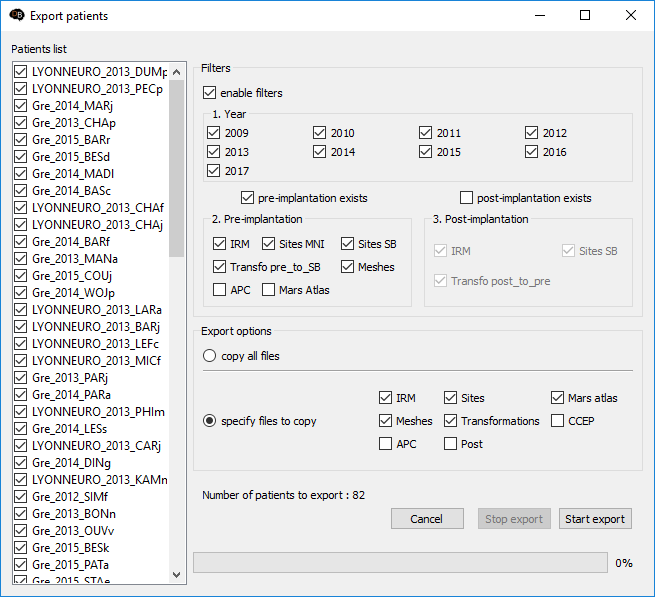
\includegraphics[scale=0.5]{ExportPatient.png}
\end{center}
\caption{\label{dbManagerExportPatient}Export patients window}
\end{figure}
\subsubsection{Functional data}\label{exportFunctional}
\paragraph{} Exporting functional data is very similar to exporting anatomical data (Figure \ref{dbManagerExportLoca}).
\begin{figure}[H]
\begin{center}
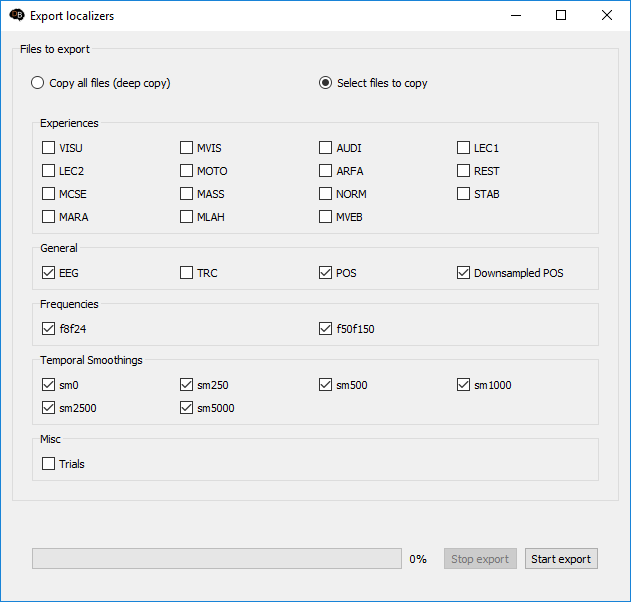
\includegraphics[scale=0.5]{ExportLoca.png}
\end{center}
\caption{\label{dbManagerExportLoca}Export localizers window}
\end{figure}
\subsection{Resources files}
\paragraph{} A folder called "resources" is present next to the executable of the DB Manager. It contains useful files for the DB Manager to work. These files can either be edited using a text editor or, for some files only, you can edit them safely using Settings/Edit experiences sub-menu. They contain:
\begin{itemize}
\item \textbf{broadman\_areas.txt}: links between the name of a broadman area and its respective index
\item \textbf{corr\_nomenclature.txt}: links between the names of the same patient in the anatomical database (right) and in the functional database (left)
\item \textbf{Downsamplings.txt}: list of possible values for the downsamplings
\item \textbf{Experiences.txt}: list of experiences to find in the functional database
\item \textbf{Frequencies.txt}: list of possible values for frequency ranges
\item \textbf{localizers.tsv}: metadata for the localizers used to convert the database to BIDS
\item \textbf{mars\_atlas\_index.csv}: links between the name of a mars atlas area and its respective index
\item \textbf{TemporalSmoothings.txt}: list of possible values for the temporal smoothings
\item \textbf{Years.txt}: list of possible values for the years
\item \textbf{Images localizers}: this folder contains illustrations for the localizers (these images are exported into the HiBoP project created with the DB Manager)
\item \textbf{Protocols}: this folder contains .prov files readable by HiBoP to describe the localizers (these protocol files are exported into the HiBoP project created with the DB Manager)
\end{itemize}
\section{HiBoP Database Hierarchy}\label{bddhierarchy}
\paragraph{} In order to use HiBoP and the DB Manager with automatic loading of patients, a specific hierarchy of the database must be respected. There is a specific hierarchy for the anatomical database (usable in both HiBoP and the Database Manager) and for the functional database (usable only in the Database Manager). These are presented in the following sections. Note that BIDS format will be supported in a near future.
\subsection{Anatomical database}
\begin{figure}[H]
\framebox[\textwidth]{%
\begin{minipage}{0.9\textwidth}
\dirtree{%
	.1 Database/.
	.2 <PATIENT>/.
	.3 implantation/.
	.4 <PATIENT>.pts.
	.4 <PATIENT>\_MNI.pts.
	.4 <PATIENT>\_ACPC.pts.
	.4 <PATIENT>.csv.
	.3 t1mri/.
	.4 T1pre\_<DATEFULL>/.
	.5 <PATIENT>.nii.
	.5 registration/.
	.6 RawT1-<PATIENT>\_T1pre\_<DATEFULL>\\\_TO\_Scanner\_Based.trm.
	.5 default\_analysis/.
	.6 segmentation/.
	.7 mesh/.
	.8 <PATIENT>\_Lhemi.gii.
	.8 <PATIENT>\_Rhemi.gii.
	.8 <PATIENT>\_Lwhite.gii.
	.8 <PATIENT>\_Rwhite.gii.
	.8 surface\_analysis/.
	.9 <PATIENT>\_Lwhite\_parcels\\\_marsAtlas.gii.
	.9 <PATIENT>\_Rwhite\_parcels\\\_marsAtlas.gii.
	.4 T1post\_<DATEFULL>/.
	.5 <PATIENT>.nii.
	.5 registration/.
	.6 RawT1-<PATIENT>\_T1post\_<DATEFULL>\\\_TO\_Scanner\_Based.trm.
}
\end{minipage}
}
\caption{\label{patientsHierarchy}Anatomical database hierarchy}
\end{figure}
\paragraph{} On the figure \ref{patientsHierarchy}:
\begin{itemize}
\item \textbf{<PATIENT>} corresponds to the patient ID, which is of the form\\<PLACE>\_<DATE>\_<NAME> (e.g. LYONNEURO\_2014\_THUv)
\item \textbf{<PLACE>} is where the patient data comes from (e.g. LYONNEURO)
\item \textbf{<DATE>} is the year the data has been acquired (e.g. 2014)
\item \textbf{<NAME>} is the anonymized name of the patient (e.g. THUv)
\item \textbf{<DATEFULL>} is the complete date (e.g. 2015-5-20)
\end{itemize}
\subsection{Functional database}
\begin{figure}[H]
\framebox[\textwidth]{%
\begin{minipage}{0.9\textwidth}
\dirtree{%
	.1 Database/.
	.2 <DATE>/.
	.3 <LOCA>/.
	.4 <LOCA>.TRC.
	.4 <LOCA>.eeg.
	.4 <LOCA>.eeg.ent.
	.4 <LOCA>.pos.
	.4 <LOCA>\_<DS>.pos.
	.4 <LOCA>\_<FF>/.
	.5 <LOCA>\_<FF>\_<DS>\_<SM>.eeg.
	.5 <LOCA>\_<FF>\_<DS>\_<SM>.eeg.ent.
	.5 <LOCA>\_<FF>\_trials/.
	.6 <LOCA>\_<FF>\_<DS>\_<SM>\_trials\_<SITE>.jpg.
}
\end{minipage}
}
\caption{\label{locasHierarchy}Functional database hierarchy}
\end{figure}
\paragraph{} The figure \ref{locasHierarchy} explains the hierarchy for the data we commonly use. It may not be adapted to every kinds of iEEG data. On this figure:
\begin{itemize}
\item \textbf{<LOCA>} is the name of the localizer which is usually of the form\\<PATIENT>\_<EXP> (e.g. LYONNEURO\_2014\_THUV\_LEC1).\\<PATIENT> is usually the same as in the anatomical database; if their names are different (case sensitive), you need to create a link in the corr\_nomenclature.txt file of the DB Manager if you wish to use this database with the DB Manager.
\item \textbf{<PATIENT>} corresponds to the patient ID, which is of the form\\<PLACE>\_<DATE>\_<NAME> (e.g. LYONNEURO\_2014\_THUv)
\item \textbf{<PLACE>} is where the patient data comes from (e.g. LYONNEURO)
\item \textbf{<DATE>} is the year the data has been acquired (e.g. 2014)
\item \textbf{<NAME>} is the anonymized name of the patient (e.g. THUv)
\item \textbf{<FF>} is the frequency range of the processed data (e.g. f8f24 for alpha-beta or f50f150 for gamma)
\item \textbf{<DS>} is the downsampling frequency of the processed data (e.g. ds8, ds16 or ds32)
\item \textbf{<SM>} is the temporal smoothing of the processed data (e.g. sm0, sm250, sm500, sm1000, sm2500 or sm5000)
\item \textbf{<SITE>} is the name of the channel (e.g. E5)
\end{itemize}
\end{document}